
% Mikes: ok
% Spellcheck: ok

% ============================================================
\chapter{Financial Calculations and Modeling}{}{}
\label{ch:business}
 
\index{data analysis!financial calculations|(} 
\index{financial calculations|(}  
    
\Fint{I recently received a notice from a magazine reminding me that my
subscription was running out}. It's a relatively expensive weekly
magazine, and they offered me three different plans to renew my
subscription: one year (52 issues) for \$130, two years for \$220, or
three years for \$275.  Table \ref{tbl:subscriptions} summarizes these
options and also shows the respective cost per issue.

\begin{table}[h]
\def\vrl{\smash{\vrule height54pt  width.25pt depth4pt}}
\tbl{Pricing plans for a magazine subscription\label{tbl:subscriptions}}{%
\begin{tabular}{l@{\hskip9pt}c@{\hskip9pt}c@{\hskip9pt}c@{\hskip9pt}c}
\toprule
  \TCH{Subscription} && \TCH{Total price} && \TCH{Price per issue} \\\colrule
  Single issue && n/a   && 6.00 \\
  1 year       && 130 && 2.50 \\
  2 years      && 220 && 2.12 \\
  3 years      &\vrl& 275 &\vrl& 1.76 \\\botrule
\end{tabular}}
\end{table}

Assuming that I want to continue the subscription, which of these
three options makes the most sense? From Table \ref{tbl:subscriptions},
we can see that each issue of the magazine becomes cheaper as I commit
myself to a longer subscription period, but is this a good deal?  In
fact, what does it mean for a proposal like this to be a ``good
deal''? Somehow, stomping up nearly three hundred dollars right now
seems like a stretch, even if I remind myself that it saves me more
than half the price on each issue.

This little story demonstrates the central topic of this chapter: the
\emph{time value of money}, which expresses the notion that a hundred
dollars today are worth more than a hundred dollars a year from now.
In this chapter,\vadjust{\pagebreak} I shall introduce some standard concepts and
calculational tools that are required whenever we need to make a
choice between different investment decisions---whether they involve
our own personal finances or the evaluation of business cases for
different corporate projects.

I find the material in this chapter fascinating---not because it is
rocket science (it isn't) but because it is so fundamental to how the
economy works. Yet very few people, in particular, very few tech
people, have any understanding of it. (I certainly didn't.) This is a
shame, not just because the topic is obviously important but also
because it is not really all that mystical. A little familiarity with
the basic concepts goes a long way toward removing most of the
confusion (and, let's face it, the intimidation) that many of us
experience when reading the Wall Street pages.

More important in the context of this book is that a lot of data
analysis is done specifically to evaluate different business proposals
and to support decisions among them. To be able to give effective,
appropriate advice, you want to understand the concepts and
terminology of this particular problem domain.

% ============================================================
\section{The Time Value of Money}

\index{financial calculations!time value of money|(}
\index{time value of money|(}
 
Let's return to the subscription problem. The essential insight is
that---instead of paying for the second and third year of the
subscription \emph{now}---I could invest that money, reap the
investment benefit, and pay for the subsequent years of the
subscription later. In other words, the discount offered by the
magazine must be \emph{greater} than the investment income I can
expect if I were instead to invest the sum.
    
It is this ability to gain an investment benefit that makes having
money \emph{now} more valuable than having the same amount of money
\emph{later}. Note well that this has nothing to do with the concept
of \emph{inflation}, which is the process by which a certain amount of
money tends to buy a lesser amount of goods as time passes. For our
purposes, inflation is an external influence over which we have no
control. In contrast, investment and purchasing decisions (such as the
earlier magazine subscription problem) are under our control, and time
value of money calculations can help us make the best possible
decisions in this regard.

\subsection{A Single Payment: Future and Present Value}
 
\index{time value of money!future and present value}  
\index{future value}
\index{present value}
  
Things are easiest when there is only a single payment involved.
Imagine we are given the following choice: receive \$1,000 today, or
receive \$1,050 a year from now. Which one should we choose?
    
Well, that depends on what we could do with \$1,000 right now.  For
this kind of analysis, it is customary to assume that we\vadjust{\pagebreak} would put
the money in a ``totally safe form of investment'' and use the returns
generated\vadjust{} in this way as a benchmark for comparison.\footnote{This
  used to mean investing in U.S.\ Treasury Bonds or the equivalent,
  but at the time of this writing, even these are no longer considered
  sacrosanct. But that's leaving the scope of this discussion!} Now we
can compare the alternatives against the interest that would be
generated by this ``safe'' investment. For example, assume that the
current interest rate that we could gain on a ``safe'' investment is 5
percent annually. If we invest \$1,000 for a full year, then at the
year's end, we will receive back our principal (\$1,000) and, in
addition, the accrued interest ($0.05 \cdot \$1000 = \$50$), for a
total of \$1,050.
    
In this example, both options lead to the same amount of money after
one year; we say that they are \emph{equivalent}. In other words,
receiving \$1,000 now is \emph{equivalent} to receiving \$1,050 a year
from now, \emph{given} that the current interest rate on a safe form
of investment is 5 percent annually. Equivalence always refers to a
specific time frame and interest rate.
    
Clearly, any amount of money that we now possess has a \emph{future
  value} (or \emph{future worth}) at any point in the future;
likewise, a payment that we will receive at some point in the future
has a \emph{present value} (or \emph{present worth}) now.  Both values
depend on the interest rate that we could achieve by investing in a
safe alternative investment instead. The present or future values must
be equivalent at equal times.

%%% XXX is the last statement exactly right? #
    
There is a little bit of math behind this that is not complicated but
is often a little messy. The future value $V_f$ of some base amount
$M$ (the \emph{principal}), after a single time period during which
the amount earns $p$ percent of interest, is calculated as follows:
%
\begin{align*}
V_f & = M + \frac{p}{100} M \\
    & = \paren{ 1 + \frac{p}{100} } M
\end{align*}
%
The first term on the righthand side expresses that we get our
principal back, and the second term is the amount of interest we
receive in addition. Here and in what follows, I explicitly show
the denominator 100 that is used to translate a statement such as
``$p$ percent'' into the equivalent numerical factor $p/100$.
    
Conversely, if we want to know how much a certain amount of money in
the future is worth today, then we have to \emph{discount} that amount
to its present value. To find the present value, we work the preceding
equation backward. The present value $V_p$ is unknown, but we do know
the amount of money $M$ that we will have at some point in the future,
hence the equation becomes:
%
\[
M = \paren{ 1 + \frac{p}{100} } V_p
\]
%    
This can be solved for $V_p$:
%
\[
V_p = \frac{M}{1+\frac{p}{100}}
\]
%   
Note how we find the future or present value by multiplying the base
amount by an appropriate \emph{equivalencing factor}---namely, the
future-worth factor $1+p/100$ and the present-worth factor
$1/(1+p/100)$. Because most such calculations involve discounting a
future payment to the present value, the percentage rate $p$ used in
these formulas is usually referred to as the \emph{discount rate}.
    
This example was the simplest possible because there was only a single
payment involved---either at the beginning or at the end of the period
under consideration. Next, we look at scenarios where there are
multiple payments occurring over time.

\subsection{Multiple Payments: Compounding}

\index{time value of money!compounding|(}
\index{compounding|(}
    
Matters become a bit more complicated when there is not just a single
payment involved as in the example above but a series of payments
over time. Each of these payments must be discounted by the
appropriate time-dependent factor, which leads us to \emph{cash-flow
  analysis}. \index{cash-flow analysis} In addition, payments made or received may alter the
base amount on which we operate, this leads to the concept of
\emph{compounding}.

Let's consider compounding first, since it is so fundamental. Again,
the idea is simple: if we put a sum of money into an interest-bearing
investment and then \emph{reinvest} the generated interest, we will
start to receive interest on the interest itself. In other words, we
will start receiving \emph{compound interest}.

Here is how it works: we start with principal $M$ and invest it
at interest rate $p$. After one year, we have:
%
\[
V(1) = \left( 1 + \frac{p}{100} \right) M
\]
%  
In the second year, we receive interest on the combined sum of the
principal and the interest from the first year:
%
\begin{align*}
V(2) & = \left( 1 + \frac{p}{100} \right) V(1) \\
     & = \left( 1 + \frac{p}{100} \right)^2 M
\end{align*}
%
and so on. After $n$ years, we will have:
%
\[
V(n) = \left( 1 + \frac{p}{100} \right)^n M
\]
%    
These equations tell us the future worth of our investment at any
point in time. It works the other way around, too: we can determine
the present value of a payment that we expect to receive $n$ years
from now by working the equations backward (much as we did previously
for a single payment) and find:
%
\[
V(\text{present}) = \frac{M}{ \left( 1+\frac{p}{100} \right)^n }
\]
%    
We can see from these equations that, if we continue to reinvest our
earnings, then the total amount of money grows exponentially with time
(\ie, as $a^t$ for some constant $a$)---in other words,
\emph{fast}. The growth law that applies to compound interest is the
same that describes the growth of bacteria cultures or similar
systems, where at each time step new members are added to the
population \emph{and} start producing offspring themselves. In such
systems, not only does the population grow, but the rate at which it
grows is constantly increasing as well.
    
On the other hand, suppose you take out a loan without making payments
and let the lender add the accruing interest back onto your principal.
In this case, you not only get deeper into debt every month, but you
do so at a faster rate as time goes by.

\subsection{Calculational Tricks with Compounding}
    
Here is a simple trick that is quite convenient when making
approximate calculations of~future and present worth. The
single-payment formula for future worth, $V = (1+p/100) M$, is simple
and intuitive: the principal \emph{plus} the interest after one
period. In contrast, the corresponding formula for present worth $V =
\frac{M}{1+p/100}$, seems to make less intuitive sense and is harder
to work with (how much is \$1,000 divided by 1.05?). But this is again
one of those situations where guesstimation techniques (see Chapter
\ref{ch:guesstimation}; also see Appendix \ref{app:calculus}) can be
brought to bear. We can approximate the discounting factor as follows:
%
\[
\frac{1}{1+\frac{p}{100}} 
  \approx 1 - \frac{p}{100} + \left( \frac{p}{100} \right)^2 \mp \dotsb
\]
%    
Since $p$ is typically small (single digits), it follows that $p/100$
is very small, and so we can terminate the expansion after the first
term. Using this approximation, the discounting equation for the
present worth becomes $V = ( 1 - p/100 ) M$, which has an intuitive
interpretation: the present value is equal to the future value, less
the interest that we will have received by then.
    
We can use similar formulas even in the case of compounding, since:
%
\begin{gather*}
\left( 1 + \frac{p}{100} \right)^n \approx 1 + n \frac{p}{100} + \dotsb \\
\left( 1 + \frac{p}{100} \right)^{-n} \approx 1 - n \frac{p}{100} + \dotsb 
\end{gather*}
%
However, keep in mind that the overall perturbation must be small for
the approximation to be valid. In particular, as the number of years
$n$ grows, the perturbation term $n p/100$ may no longer be small.
Still, even for 5 percent over 5 years, the approximation gives $1 \pm
25/100 = 1.25$ or 0.75, respectively. Compare this with the exact
values of 1.28 and 0.79.  However, for 10 percent over 10 years, the
approximation starts to break down, yielding 2 and 0, respectively,
compared to the exact values of 2.59 and 0.39.
    
Similar logic is behind ``Einstein's Rule of 72.'' This rule of thumb
states that if you divide 72 by the applicable interest rate, you
obtain the number of years it would take for your investment to
double.  So if you earn 7 percent interest, your money will double in
10 years, but if you only earn 3.5 percent, it will take 20 years to
double.
    
What's the basis for this rule? By now, you can probably figure it out
yourself, but here is the solution in a nutshell: for your investment
to double, the compounding factor must equal 2. Therefore, we need to
solve $(1 + p/100)^n = 2$ for $n$. Applying logarithms on both sides
we find $n = \log(2)/\log(1+p/100)$. In a second step, we expand the
logarithm in the denominator (remember that $p/100$ is a small
perturbation!) and end up with $n = \log(2) \cdot (100/p) = 69/p$,
since the value of $\log(2)$ is approximately 0.69. The number 69 is
awkward to work with, so it is usually replaced by the number
72---which has the advantage of being evenly divisible by 2, 3, 4, 6,
8, and 9 (you can replace 72 with 70 for interest rates of 5 or 7
percent).
    
Here is another calculational tool that you may find useful.  Strictly
speaking, an expression such as $x^n$ is defined only for integer
$n$. For general exponents, the power function is defined as $x^n =
\exp(n \log x)$. We can use this when calculating compounding factors
as follows:
%
\begin{align*}
\paren{ 1 + \frac{p}{100} }^n 
  & = \exp \paren{ n \log \paren{1 + p/100} } \\
  & \approx e^{n p/100}
\end{align*}
%    
where in the second step we have expanded the logarithm again and
truncated the expansion after the first term. This form of the
compounding factor is often convenient (\eg, it allows us to use
arbitrary values for the time period $n$, not just full years). It
becomes exact in the limit of continuous compounding (discussed
shortly).
    
Interest rates are conventionally quoted ``per year,'' as in ``5
percent annually.'' But payments may occur more frequently than that.
Savings accounts, for example, pay out any accrued interest on a
monthly basis. That means that (as long as we don't withdraw anything)
the amount of money that earns us interest grows every month; we say
it is \emph{compounded monthly}. (This is in contrast to other
investments, which pay out interest or dividends only on a quarterly
or even annual basis.) To take advantage of the additional
compounding, it is of course in our interest (pun intended) to receive
payments as early as possible.
  
This monthly compounding is the reason for the difference between the
\emph{nominal} interest rate and the annual \emph{yield} that you will
find stated on your bank's website: the nominal interest rate is the
rate $p$ that is used to determine the amount of interest paid
out to you each month. The yield tells you by how much your money will
grow over the course of the year when the monthly compounding has
been factored in. With our knowledge, we can now calculate the yield
from the nominal rate:
%
\[
\left( 1 + \frac{p_{{\rm yield}}}{100} \right) 
 = \left( 1 + \frac{ \frac{p_{{\rm nominal}}}{12}}{100} \right)^{12} 
\]
%
One more bit of terminology: the interest rate $p/12$ that is used to
determine the value of the monthly payout is known as the
\emph{effective} interest rate.
    
Of course, other payment periods are possible. Many mutual funds pay
out quarterly. In contrast, many credit cards compound daily.  In
theory, we can imagine payments being made constantly (but at an
appropriately reduced effective interest rate); this is the case of
\emph{continuous compounding} mentioned earlier. In this case, the
compounding factor is given by the exponential function.
(Mathematically, you replace the 12 in the last formula by $n$ and
then let $n$ go to infinity, using the identity $\lim_{n \to \infty}
(1 + x/n)^n = \exp(x)$.)

\index{time value of money!compounding|)}
\index{compounding|)}

\subsection{The Whole Picture: Cash-Flow Analysis and Net Present Value}

\index{time value of money!cash-flow analysis and net present value|(}
\index{cash-flow analysis|(}
\index{NPV (net present value)|(} 
\index{net present value NPV)|(} 
 
We now have all the tools at our disposal to evaluate the financial
implications of any investment decision, no matter how complicated.
Imagine we are running a manufacturing plant (or perhaps an operation
like Amazon's, where books and other goods are put into boxes and
mailed to customers---that's how \emph{I} learned about all these
things). We may consider buying some piece of automated equipment for
some part of the process (\eg, a sorting machine that sorts boxes onto
different trucks according to their destination).  Alternatively, we
can have people do the same job manually.  Which of these two
alternatives is better from an economic point of view?
    
The manual solution has a simple structure: we just have to pay out
the required wages every year. If we decide to buy the machine, then
we have to pay the purchase price now (this is also known as the
\emph{first cost}) and also pay a small maintenance fee each year. For
the sake of the argument, assume also that we expect to use the
machine for ten years and then sell it on for scrap value.
    
In economics texts, you will often find the sequence of payments
visualized using \emph{cash-flow diagrams} (see Figure
\ref{fig:cashflow}). Time progresses from left to right; inflows are
indicated by upward-pointing arrows and outflows by downward-pointing
arrows.

% omitting revenue : assumed the same for both solutions 

\begin{figure}
  \centerline{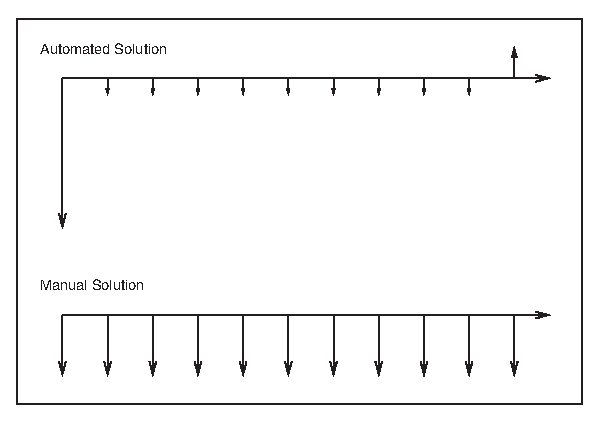
\includegraphics{img/cashflow}}
  \caption{Examples of cash-flow diagrams. Arrows pointing up
    correspond to money received; arrows pointing down, to money
    spent.}
  \label{fig:cashflow}
\end{figure}
    
To decide between different alternatives, we now proceed as follows:

\begin{enumerate}
\item Determine all individual net cash flows (\emph{net} cash flows, 
  because we offset annual costs against revenues).
\item Discount each cash flow to its present value.
\item Add up all contributions.
\end{enumerate}
 
The quantity obtained in the last step is known either as the
\emph{net present value} (NPV) or the \emph{discounted net cash flow}:
it is the total value of all cash flows, each properly discounted to
its present value. In other words, our financial situation will be the
same, whether we execute the entire series of cash flows \emph{or}
receive the net present value today.  Because the net present value
contains all inflows and outflows (properly discounted to the present
value), it is a comprehensive single measure that can be used to
compare the financial outcomes of different investment strategies.

We can express the net present value of a series of cash flows in a
single formula:
%
\[
\text{NPV} = \sum_i \frac{c(i)}{(1+p/100)^i}
\]
%
where $c(i)$ is the net cash flow at payment period $i$ and
$1/(1+p/100)^i$ is the associated discounting factor.

% --- XXX : is this at all clear?

There is one more concept that is interesting in this context. What
should we use for the discount rate $p$ in the second step above?
Instead of supplying a value, we can ask how much interest we would
have to receive elsewhere (on a ``safe'' investment) to obtain the
same (or higher) payoff than that expected from the planned project.
Let's consider an example. Assume we are evaluating a project that
would require us to purchase some piece of equipment at the beginning
but that would then result in a series of positive cash flows over the
next so many years.  Is this a ``good'' investment? It is if its net
present value is positive! (That's pretty much the definition of ``net
present value'': the NPV takes into account the first cost to purchase
the equipment as well as the subsequent positive cash flows. If the
discounted cash flows are greater than the first cost, we come out
ahead.) But the net present value depends on the discount rate $p$, so
we need to find that value of $p$ for which the NPV first becomes
zero: if we can earn a higher interest rate elsewhere, then the
project does not make financial sense and we should instead take our
money to the bank. But if the bank would pay us less than the
\emph{rate of return} just calculated, then the project is financially
the better option. (To find a numeric value for the rate of return,
plug your cash flow structure $c(i)$ into the equation for NPV and
then solve for $p$. Unless the cash flows are particularly simple, you
will have to do this numerically.)

The net present value is such an important criterion when making
investment decisions because it provides us with a single number that
summarizes the financial results of any planned project. It gives us
an objective (financial) quantity to decide among different investment
alternatives.
    
Up to a point, that is. The process described here is only as good as
its inputs. In particular, we have assumed that we know all inputs
perfectly---possibly for many years into the future.  Of course we
don't have perfect knowledge, and so we better accommodate for that
uncertainty somehow. That will be the topic of the next section.
    
There is another, more subtle problem when evaluating different
options solely based on net present value: different investment
alternatives may have nonfinancial benefits or drawbacks that are not
captured by the net present value.  For example, using manual labor
may lead to greater flexibility: if business grows more strongly than
expected, then the company can hire additional workers, and if
business slows down, then it can reduce the number of workers. In
contrast, any piece of equipment has a maximum capacity, which may be
a limiting factor if business grows more strongly than expected. The
distinction arising here is that between fixed and variable cost, and
we will come back to it toward the end of the chapter.

\index{time value of money!cash-flow analysis and net present value|)}
\index{cash-flow analysis|)}
\index{NPV (net present value)|)} 
\index{net present value NPV)|)} 
\index{financial calculations!time value of money|)}
\index{time value of money|)}

\vspace*{-9pt}
% ============================================================
\section{Uncertainty in Planning and Opportunity Costs}

\index{financial calculations!uncertainty and opportunity costs|(} 
\index{uncertainty in planning|(}
     
Now we are ready to revisit the magazine subscription problem from the
beginning of this chapter. Let's consider only two alternatives:
paying the entire amount for a two-year subscription up front or
making two single-year payments. The NPV for the second option is
$\left( 1 + 1/(1+p/100) \right) C_{{\rm 1yr}}$, where we have left
the discount rate $p$ undetermined for the moment. We can now ask:
what interest rate would we have to earn elsewhere to make the second
option worthwhile? In other words, we want to know the discount rate
we'd have to apply to make the NPV of the multiple-payment option
equal to the cost of the single-payment plan:
%
\[
\left( 1 + \frac{1}{1+\frac{p}{100}} \right) C_{{\rm 1yr}} = C_{{\rm 2yr}}
\]
%    
This equation can be solved for $p$. The result is $p = 30$ percent!
In other words, the two-year subscription is so much cheaper that we
would have to find an investment yielding 30 percent annually before
it would be worthwhile to pay for the subscription year by year and
invest the saved money elsewhere. No investment (and certainly no
``safe'' investment) yields anywhere near that much. Clearly,
something is amiss. (Exercise for the reader: find the net present
value for the three-year subscription and verify that it leads to the
same value for $p$.)

\vspace*{-6pt}
\subsection{Using Expectation Values to Account for Uncertainty}

\index{expectation values!accounting for uncertainty}
 
The two- and three-year plans carry a hidden cost for us: once we have
signed up, we can no longer freely\vadjust{\pagebreak} decide over our money---we're
committed ourselves for the long haul. In contrast, if we pay on a
yearly basis, then we can reevaluate every year whether we want to
continue the subscription.  The price for this freedom is a higher
subscription fee. However, we will probably not find it easy to
determine the exact dollar value that this freedom is worth to us.
    
From the magazine's perspective, the situation is simpler. They can
simply ask how much money they expect to make from an individual
subscriber under either option. If I sign up for the two-year
subscription, they make $C_{{\rm 2yr}}$ with certainty; if I sign up
for the one-year subscription, they make $C_{{\rm 1yr}}$ with
certainty now and another $C_{{\rm 1yr}}$ later---\emph{provided} I
renew my subscription! In this case, then, the amount of money the
magazine expects to make on me is $C_{{\rm 1yr}} + \gamma
C_{{\rm 1yr}}$, where $\gamma$ is the probability that I will renew
the subscription. From the magazine's perspective, both options must
be equally favorable (otherwise they would adjust the price of the
two-year subscription to make them equal), so we can equate the
expected revenues and solve for $\gamma$. The result comes out to
about $\gamma = 0.7$---in other words, the magazine expects (based on
past experience, and so on) that about 70 percent of its current
subscribers will renew their subscription. For three years, the
equation becomes $( 1 + \gamma + \gamma^2) C_{{\rm 1yr}} =
C_{{\rm 3yr}}$ because, to sign up for three years, a subscriber must
decide \emph{twice} to renew the subscription. If you work through the
algebra, you will find that $\gamma$ again comes out to about $\gamma
= 0.7$, providing a nice consistency check.

There are two takeaways in this example that are worth emphasizing:
the first concerns making economic decisions that are subject to
uncertainty. The second is the concept of opportunity cost, which is
the topic of the following section.

When making economic decisions that are subject to uncertainty, you
may want to take this uncertainty into account by replacing the
absolute cash flows with their expected values. A simple probability
model for the likely payout is often sufficient.  In the magazine
example there were just two outcomes: the subscriber renews with
probability $\gamma = 0.7$ and value $C_{{\rm 1yr}}$, or the
subscriber does not renew with probability $\gamma = 0.3$ and value
$0$, hence the expected value is $0.3 \cdot 0 + 0.7 \cdot
C_{{\rm 1yr}}$. If your situation warrants it and if you can specify
the probability distribution for various payout alternatives in more
detail, then you can calculate the expected value accordingly. (See
Chapter \ref{ch:scaling} and Chapter \ref{ch:probability} for more
information on how to build models to support this kind of
conclusion.)

% Below: do I need to be more explicity on the simulation topic?
    
Working with expectation values is convenient, because once you have
determined the expected value of the payout, you no longer need to
worry about the probabilities for the various outcomes: they have been
entirely absorbed into the expectation values. What you lose is
insight into the probable spread of outcomes. For a quick
order-of-magnitude check, that's acceptable, but for a more serious
study, an estimate of the spread should be included.  There are two
ways to do this: repeat your calculation multiple times using
different values (low, medium, high) for the expected payouts at every
step to develop a sense for the range of possible outcomes. (If there
are many different options, you may want to do this through
simulation; see\vadjust{\pagebreak} Chapter \ref{ch:simulation}.) Alternatively, you can
evaluate both the expectation value and the spread directly from the
probability distribution to obtain a range for each estimated value:
$\mu \pm \sigma$.  Now you can use this sum in your calculations,
treating $\sigma$ as a small perturbation and evaluate the effect of
this perturbation on your model (see Chapter \ref{ch:guesstimation}).

\index{uncertainty in planning|)}

\vspace*{-6pt}
\subsection{Opportunity Costs}

\index{opportunity costs}
\index{costs!opportunity costs}
   
The second point that I would like to emphasize is the concept of
\emph{opportunity cost}. Opportunity costs arise when we miss out on
some income (the ``opportunity'') because we were not in a position to
take advantage of it. Opportunity costs formalize the notion that
resources are finite and that, if we apply them to one purpose, then
those resources are not available for other uses. In particular, if we
commit resources to a project, then we want that project to generate a
benefit greater than the opportunity costs that arise, because those
resources are no longer available for other uses.
    
I find it easiest to think about opportunity cost in the context of
certain business situations.  For instance, suppose a company takes on
a project that pays \$15,000.  While this contract is under way,
someone else offers the company a project that would pay
\$20,000. Assuming that the company cannot break its initial
engagement, it is now incurring an opportunity cost of \$5,000.
    
I find the \emph{concept} of opportunity cost useful as a way to put a
price on alternatives, particularly when no money changes hands. In
textbooks, this is often demonstrated by the example of the student
who takes a trip around the world instead of working at a summer job.
Not only does the student have to pay the actual expenses for the
trip but also incurs an opportunity cost equal to the amount of
forgone wages. The concept of opportunity cost allows us to account
for these forgone wages, which would otherwise be difficult because
they do not show up on any account statement (since they were never
actually paid).

On the other hand, I often find opportunity cost a somewhat shadowy
concept because it totally hinges on a competing opportunity actually
arising. Imagine you try to decide between two opportunities: an offer
for a project that would pay \$15,000 and the prospect of a project
paying \$20,000.  If you take the first job and then the second
opportunity comes through as well, you are incurring an opportunity
cost of \$5,000. But if the second project falls through, your
opportunity cost just dropped to zero! (The rational way to make this
decision would be to calculate the total revenue expected from each
prospect but \emph{weighted by the probability} that the contract will
actually be signed. This brings us back to calculations involving
\emph{expected} payouts, as discussed in the preceding section.)
    
To be clear: the concept of opportunity cost has nothing to do with
uncertainty in planning. It is merely a way to evaluate the relative
costs of competing opportunities. However, when evaluating competing
deals, we must often decide between plans that have a different
likelihood of coming to fruition, and therefore opportunity cost and
planning for uncertainty often arise together.

\index{financial calculations!uncertainty and opportunity costs|)} 

% ============================================================
\section{Cost Concepts and Depreciation}

\index{financial calculations!cost concepts and depreciation|(} 
\index{costs!cost concepts and depreciation|(}
    
The methods described in the previous sections might suggest that the
net present value is all there is to financial considerations.  This
is not so---other factors may influence our decision. Some factors are
entirely outside the financial realm (\eg, ethical or strategic
considerations); others might have direct business implications but
are not sufficiently captured by the quantities we have discussed so
far.

For example, let's go back to the situation discussed earlier where we
considered the choice between two alternatives: buying a sorting
machine or having the same task performed manually.  Once we identify
all arising costs and discount them properly to their present value,
it would seem we have accounted for all financial implications.  But
that would be wrong: the solution employing manual labor is more
flexible, for instance. If the pace of the business varies over the
course of the year, then we need to buy a sorting machine that is
large enough to handle the busiest season---which means it will be
underutilized during the rest of the year. If we rely on manual labor,
then we can more flexibly scale capacity up through temporary labor or
overtime---and we can likewise respond to unexpectedly strong (or
weak) growth of the overall business more flexibly, again by adjusting
the number of workers. (This practice may have further
consequences---for example, regarding labor relations.) In short, we
need to look at the costs, and how they arise, in more detail.

To understand the cost structure of a business or an operation better,
it is often useful to discuss it in terms of three pairs of
complementary concepts:

\begin{enumerate}
\item Direct versus indirect cost
\item Fixed versus variable cost
\item Capital expenditure versus operating cost
\end{enumerate}

For good measure, I'll also throw in the concept of
\emph{depreciation}, although it is not a cost in the strict sense of
the word.

\subsection{Direct and Indirect Costs}

\index{direct costs}
\index{indirect costs}
  
Labor and materials that are applied in creating the \emph{product}
(\ie, in the creation of something the company will \emph{sell}) are
considered direct labor or direct materials cost.  Indirect costs, on
the other hand, arise from activities that the company undertakes
to maintain \emph{itself}: management, maintenance, and administrative
tasks (payroll and accounting) but also training, for example. Another
term for such indirect costs is \emph{overhead}.

I should point out that this is a slightly different definition of
direct and indirect costs than the one you will find in the
literature. Most textbooks define direct cost as the cost that is
``easily attributable'' to the production process, whereas indirect
cost is ``not easily attributable.'' This definition makes\vadjust{\pagebreak} it seem as
if the distinction between direct and indirect costs is mostly one of
convenience. Furthermore, the textbook definition provides no reason
why, for example, maintenance and repair activities are usually
considered indirect costs. Surely, we can keep track of which machine
needed how much repair and therefore assign the associated cost to the
product made on that specific machine. On the other hand, by my
definition, it is clear that maintenance should be considered an
indirect cost because it is an activity the company undertakes to keep
\emph{itself} in good order---not to generate value for the customer.

I have used the term ``product'' for whatever the company is selling.
For manufacturing or retail industries this is a straightforward
concept, but for a service industry the ``product'' may be intangible.
Nevertheless, in probably all businesses we can introduce the concept
of a single produced unit or \emph{unit of production}. In
manufacturing and retail there are actual ``units,'' but in other
industries the notion of a produced unit is a bit more artificial: in
service industries, for instance, one often uses ``billable hours'' as
a measure of production.  Other industries have specialized
conventions: the airline industry uses ``passenger miles,'' for
example.

The unit is an important concept because it is the basis for the most
common measure of productivity---namely the unit cost or \emph{cost
  per unit} (CPU). \index{CPU (cost per unit)} The cost per unit is obtained by dividing the
total (dollar) amount spent during a time period (per month, for
instance) by the total number of units produced during that time. If
we include not only the direct cost but also the indirect cost in this
calculation, we obtain what is called the \emph{loaded} or
\emph{burdened} cost per unit.

We can go further and break out the various contributions to the unit
cost. For example, if there are multiple production steps, then we can
determine how much each step contributes to the total cost. We can
also study how much indirect costs contribute to the overall cost as
well as how material costs relate to labor. Understanding the
different contributions to the total cost per unit is often a
worthwhile exercise because it points directly to where the money is
spent. And appearances can be deceiving. I have seen situations where
literally hundreds of people were required for a certain processing
step whereas, next door, a single person was sufficient to oversee a
comparable but highly automated process. Yet once you calculated the
cost per unit, it all looked very different: because the number of
units going through the automated process was low, its total cost per
unit was actually higher than for the manual process. And because so
many units where processed manually, their labor cost \emph{per unit}
turned out to be very low.

In general, it is desirable to have low overhead relative to the
direct cost: a business should spend relatively less time and money on
managing itself than on generating value for the customer. In this
way, the ratio of direct to indirect cost can be a telling indicator
for ``top-heavy'' organizations that seem mostly occupied with
managing themselves. On the other hand, overeager attempts to improve
the direct/indirect cost ratio can lead to pretty unsanitary
manipulations. For example, imagine a company that considers software
engineers \emph{direct} labor, while\vadjust{\pagebreak} any form of management (team
leads and project managers) is considered \emph{indirect}. The natural
consequence is that management responsibilities are pushed onto
developers to avoid ``indirect'' labor. Of course, this does not make
these tasks go away; they just become invisible. (It also leads to the
inefficient use of a scarce resource: developers are always in short
supply---and they are expensive.)  In short, beware the danger of
perverted incentives!

\subsection{Fixed and Variable Costs}

\index{fixed costs}
\index{variable costs}
  
Compared to the previous distinction (between direct and indirect
costs), the distinction between fixed and variable costs is clearer. The
\emph{variable} costs are those that change in response to changing
demand, while \emph{fixed} costs don't. For a car manufacturer, the
cost of steel is a variable cost: if fewer cars are being built, less
steel is consumed. Whether labor costs are fixed or variable depends
on the type of labor and the employment contracts.  But the capital
cost for the machines in the production line is a fixed cost, because
it has to be paid regardless of whether the machines are busy or idle.

It is important not to confuse direct and variable costs.  Although
direct costs are more likely to be variable (and overhead, in general,
is fixed), these are unrelated concepts; one can easily find examples
of fixed, yet direct costs. For example, consider a consultancy with
salaried employees: their staff of consultants is a \emph{direct}
cost, yet it is also a \emph{fixed} cost because the consultants
expect their wages regardless of whether the consultancy has projects
for them or not. (We'll see another example in a moment.)

In general, having high fixed costs relative to variable ones makes a
business or industry less flexible and more susceptible to downturns.
An extreme example is the airline industry: its cost structure is
almost exclusively fixed (pretty much the only variable cost is the
price of the in-flight meal), but its demand pattern is subject to
extreme cyclical swings.

The numbers are interesting. Let's do a calculation in the spirit of
Chapter \ref{ch:guesstimation}. A modern jet airplane costs about
\$100M new and has a useful service life of about 10 years. The cost
attributable to a single 10-hour transatlantic flight (the
depreciation---see below) comes to about \$30k (\ie,
$\text{\$100M}/(10\cdot365)$---half that, if the plane is turned
around immediately, completing a full round-trip within 24 hours).
Fuel consumption is about 6 gallons per mile; if we assume a fuel
price of \$2 per gallon, then the 4,000-mile flight between New York
and Frankfurt (Germany) will cost \$50k for fuel. Let's say there are
10 members of the cabin crew at \$50k yearly salary and two people in
the cockpit at \$150k each. Double these numbers for miscellaneous
benefits, and we end up with about \$2M in yearly labor costs, or \$10k
attributable to this one flight. In contrast, the cost of an in-flight
meal (wholesale) is probably less than \$10 per person.  For a flight
with 200 passengers, this amounts to \$1,000--2,000 dollars total.  It
is interesting to see that---all things considered---the influence of
the in-flight meal on the overall cost structure of the flight is as
high as it is: about 2 percent of the total. In a business with thin
margins, improving profitability by 2 percent is usually seen as
worthwhile.\vadjust{\pagebreak}  In other words, we should be grateful that we get
\emph{anything} at all! A final cross-check: the cost per passenger
for the entire flight from the airline's point of view is \$375---and
at the time of this writing, the cheapest fare I could find was \$600
round-trip, equivalent to \$300 for a single leg.  As is well known,
airlines break even on economy class passengers but don't make any
profits.

\subsection{Capital Expenditure and Operating Cost}

\index{capital expenditures}
\index{operating costs}
  
Our final distinction is the one between \emph{capital expenditure}
(CapEx) and \emph{operating expense} (OpEx---the abbreviation is
rarely used). Capital expenses are money spent to purchase long-lived
and typically tangible assets: equipment, installations, real estate.
Operating expenses are everything else: payments for rents, raw
materials, fees, salaries. In most companies, separate budgets exist
for both types of expense, and the availability of funds may be quite
different for each. For example, in a company that is financially
strapped but does have a revenue stream, it might be quite acceptable
to hire and ``throw people'' at a problem (even at great cost), but it
might very well be impossible to buy a piece of equipment that would
take care of the problem for good. Conversely, in companies that do
have money in the bank, it is often \emph{easier} to get a lump sum
approved for a specific purchase than to hire more people or to
perform maintenance. Decision makers often are more inclined to
approve funding for an identifiable and visible purchase than for
spending money on ``business as usual.'' Political and vanity
considerations may play a role as well.

The distinction between CapEx and operating costs is important
because, depending on the availability of funds from either source,
different solutions will be seen as feasible. (I refer to such
considerations as ``color of money'' issues---although all dollars are
green, some are greener than others!)

In the context of capital expenditure, there is one more concept that
I'd like to introduce because it provides an interesting and often
useful way of thinking about money: the notion of
\emph{depreciation}.\index{depreciation}\footnote{Do not confuse \emph{to depreciate},
  which is the process by which an asset loses value over time, with
  \emph{to deprecate}, which is an expression of disapproval. The
  latter word is used most often to mark certain parts of a software
  program or library as \emph{deprecated}, meaning that they should no
  longer be used in future work.} The idea is this: any piece of
equipment that we purchase will have a useful service life. We can now
distribute the total cost of that purchase across the entire life of
the asset. For example, if I purchase a car for \$24,000 and expect to
drive it for 10 years, then I can say that this car costs me \$200 per
month ``in depreciation'' alone and before taking into account any
operating costs (such as gas and insurance). I may want to compare
this number with monthly lease payment options on the same kind of
vehicle.

In other words, depreciation is a formalized way of capturing how an
asset loses value over time. There are different standard ways to
calculate it: ``straight-line'' distributes the purchase cost (less
any \emph{salvage value} that\vadjust{\pagebreak} we might expect to obtain for the asset
at the end of its life) evenly over the service life. The ``declining
balance'' method assumes that the asset loses a certain constant
fraction of its value every year. And so on.  (Interestingly, land is
never depreciated---because it does not wear out in the way a machine
does and therefore does not have a finite service life.)

I find depreciation a useful concept, because it provides a good way
to think about large capital expenses: as an ongoing cost rather than
as an occasional lump sum. But depreciation is just that: a way of
thinking. It is important to understand that depreciation is
\emph{not} a cash flow and therefore does not show up in any sort of
financial accounting. What's in the books is the money actually spent,
when it is spent.

The only occasion where depreciation is treated as a cash flow is when
it comes to taxes. The IRS (the U.S.\ tax authority) requires that
certain long-lived assets purchased for business purposes be
depreciated over a number of years, with the annual depreciation
counted as a business expense for that year. For this reason,
depreciation is usually introduced in conjunction with tax
considerations. But I find the concept more generally useful as a way
to think about and account for the cost of assets and their declining
value over time.

\index{financial calculations!cost concepts and depreciation|)} 
\index{costs!cost concepts and depreciation|)}

% ============================================================
\section{Should You Care?}

\index{financial calculations!issues|(} 

What does all this talk about money, business plans, and investment
decisions have to do with data analysis? Why should you even care?

That depends. If you take a purely technical stance, then all of these
questions are outside your area of competence and responsibility.
That's a valid position to take, and many practitioners will make
exactly that decision.

Personally, I disagree. I don't see it as my job to provide
\emph{answers} to \emph{questions}. I see it as my responsibility to
provide \emph{solutions} to \emph{problems}, and to do this
effectively, I need to understand the context in which questions arise,
and I need to understand how answers will be evaluated and used.
Furthermore, when it comes to questions having to do with abstract
topics like data and mathematical modeling, I have found that few
clients are in a good position to ask meaningful questions.
\emph{Coaching} the client on what makes a good question (one that is
both operational for me and actionable for the client) is therefore a
large part of what I do---and to do that, I must understand and speak
the client's language.

There are two more reasons why I find it important to understand
issues such as those discussed in this (and the previous) chapter:
to establish my own \emph{credibility} and to provide advice and
counsel on the \emph{mathematical details} involved.

The decision makers---that is, the people who request and use the
results of a data analysis study---are ``business people.''  They tend
to see decisions as \emph{investment} decisions and thus will evaluate
them using the methods and terminology introduced in this chapter.
Unless I understand how they will look\vadjust{\pagebreak}  at my results and unless I can
defend my results in those terms, I will be on weak
ground---especially since I am supposed to be ``the expert.'' I
learned this the hard way: once, while presenting the results of a
rather sophisticated and involved analysis, some MBA bully fresh out
of business school challenged me with: ``OK, now which of these
options has the best discounted net cash flow?''  I had no idea what
he was talking about. I looked like an idiot.  That did \emph{not}
help my credibility! (No matter how right I was in everything else I
was presenting.)

Another reason why I think it is important to understand the concepts
in this chapter is that the math can get a little tricky. This is why
the standard textbooks resort to large collections of precooked
scenarios---which is not only confusing but can become downright
misleading if none of them fit exactly and people start combining
several of the standard solutions in ad hoc (and probably incorrect)
ways. Often the most important skill I bring to the table is basic
calculus. In one place I worked for, which was actually staffed by
some of the smartest people in the industry, I discovered a problem
because people did not fully understand the difference between $1/x$
and $-x$. Of course, if you put it like this, everybody understands
the difference. But if you muddy the waters a little bit and present
the problem in the business domain setting in which it arose, it's no
longer so easy to see the difference. (And I virtually guarantee you
that nobody will understand why $1/(1-x)$ is actually close to $1-x$
for small $x$, when $1/x$ is not equal $-x$.)

In my experience, the correct and meaningful application of basic math
outside a purely mathematical environment poses a nearly
insurmountable challenge even for otherwise very bright people.
Understanding exactly what people are trying to do (\eg, in
calculating a total rate of return) allows me to help them avoid
serious mistakes.

But in the end, I think the most important reason for mastering this
material is to be able to understand the \emph{context} in which
questions arise and to be able to answer those questions
appropriately with a sense for the \emph{purpose} driving the original
request.

\vspace*{-9pt}
% ============================================================
\section{Is This All That Matters?}

In this chapter, we discussed several financial concepts and how to use
them when deciding between different business or investment options.

This begs the question: are these the only issues that matter? Should
you automatically opt for the choice with the highest net present
value and be done with it?

Of course, the short answer is no. Other aspects matter and may even
be more important (strategic vision, sustainability, human factors,
personal interest, commitment). What makes these factors different is
that they are \emph{intangible}. You have to decide on them yourself.

The methods and concepts discussed in this chapter deal specifically
and exclusively with the \emph{financial} implications of certain
decisions. Those concerns are important---otherwise, you would not
even \emph{be} in business. But this focus should not be taken to
imply that financial considerations are the \emph{only} ones that
matter.\pagebreak

However, I am in no better position than you to give advice on ethical
questions. It's up to each of us individually---what kind of life do
we want to live?

\index{financial calculations!issues|)} 

% ============================================================
\section{Workshop: The Newsvendor Problem}

\index{financial calculations!newsvendor problem|(}
 
In this workshop, I'd like to introduce one more idea that is often
relevant when dealing with business plans and calculations on how to find
the optimal price or, alternatively, the optimal inventory level for
some item. The basic problem is often presented in the following
terms.

Imagine you run a newsstand. In the morning, you buy a certain number
$n$ of newspapers at price $c_0$. Over the course of the day, you try
to sell this inventory at price $c_1$; anything that isn't sold in the
evening is discarded (no salvage value). If you knew how many papers
you would actually sell during the course of the day (the
\emph{demand} $m$), then it would be easy: you would buy exactly $m$
papers in the morning. However, the demand is not known exactly,
although we know the probability $p(k)$ of selling exactly $k$ copies.
The question is: how many papers should you buy in the morning in
order to maximize your net earnings (the \emph{revenue})?

\begin{figure}
  \centerline{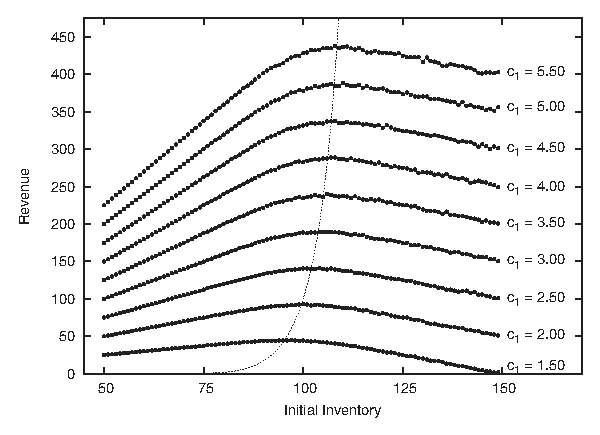
\includegraphics{img/newsboy}}
  \caption{Simulation results for the newsvendor problem: total
    revenue as a function of the initial inventory, for several values
    of the sales price $c_1$. Also shown is the (theoretical) locus of
    the initial inventory size that leads to maximum revenue.  \label{fig:newsboy}}\vspace*{-9pt}
\end{figure}

A first guess might be to use the average number of papers that we
expect to sell---that is, the mean of $p(k)$. However, this approach
may not be good enough: suppose that $c_1$ is much larger than $c_0$
(so that your markup is high). In that case, it makes sense to purchase
more papers in the hope of selling them, because\vadjust{\pagebreak}  the gain from selling
an additional paper outweighs the loss from having purchased too many.
(In other words, the \emph{opportunity cost} that we incur if we have
too few papers to satisfy all demand is greater than the cost of
purchasing the inventory.) The converse also holds: if the markup is
small, then each unsold paper significantly reduces our overall
revenue.

This problem lends itself nicely to simulations. The listing that
follows shows a minimal program for simulating the newsvendor problem.
We fix the purchase price $c_0$ at \$1 and read the projected sales
price $c_1$ from the command line. For the demand, we assume a
Gaussian distribution with mean $\mu = 100$ and standard deviation
$\sigma = 10$. Now, for each possible initial level of inventory $n$,
we make 1,000 random trials.  Each trial corresponds to a single
``day''; we randomly generate a level of demand $m$ and calculate the
resulting revenue for that day.  The revenue consists of the sales
price for the number of units that were actually sold \emph{less} the
purchase price for the inventory. You should convince yourself that
the number of units sold is the lesser of the inventory and the
demand: in the first case, we sold out; in the second case, we ended
up discarding inventory.  Finally, we average all trials for the
current level of starting inventory and print the average revenue
generated. The results are shown in Figure \ref{fig:newsboy} for
several different sales prices $c_1$:\vspace*{3pt}

\begin{verbatim}
from sys import argv
from random import gauss

c0, c1 = 1.0, float( argv[1] )
mu, sigma = 100, 10
maxtrials = 1000

for n in range( mu-5*sigma, mu+5*sigma ):
    avg = 0
    for trial in range( maxtrials ):
        m = int( 0.5 + gauss( mu, sigma ) )       
        r = c1*min( n, m ) - c0*n
        avg += r
        
    print c1, n, avg/maxtrials
\end{verbatim}

Of course, the total revenue depends on the actual sales price---the
higher the price, the more we take home. But we can also see that, for
each value of the sales price, the revenue curve has a maximum at a
different horizontal location. The corresponding value of $n$ gives us
the optimal initial inventory level for that sales price.  Thus we
have achieved our objective: we have found the optimal number of
newspapers to buy at the beginning of the day to maximize our
earnings.

This simple idea can be extended in different ways.  More complicated
situations may involve \emph{different} types of items, each with its
own demand distribution. How much of each item should we hold in
inventory now?  Alternatively, we can turn the problem around by
asking: given a fixed inventory, what would be the optimal
\emph{price} to maximize earnings? To answer this question, we need to
know how the demand varies as we change the price---that is, we need
to know the \emph{demand curve}, which takes the role of the demand
distribution in our example.

\subsection{Optional: Exact Solution}

For this particular example, involving only a single type of product
at a fixed price, we can actually work out the optimum exactly. (This
means that running a simulation wasn't strictly necessary in this
case. Nevertheless, this is one of those cases where a simulation may
actually be easier to do and less error-prone than an analytical
model. For more complicated scenarios, such as those involving
different types of items with different demands, simulations are
unavoidable.)

To solve this problem analytically, we want to find the optimum of the
expected revenue. The revenue---as we already saw in our example
simulation program---is given by
%
\[
r(m) = c_1 \min( n, m ) - c_0 n
\]
%
The revenue depends on the demand $m$. However, the demand is a random
quantity: all that we know is that it is distributed according to some
distribution $p(m)$. The \emph{expected revenue} $E[r(m)]$ is the
average of the revenue over all possible values of $m$, where each
value is weighted by the appropriate probability factor:
%
\[
E[ r(m) ] = \int_0^\infty \! r(m) \, p(m) \rms{m}
\]
%
We can now plug in the previous expression for $r(m)$, using the
lesser of $n$ and $m$ in the integral:
%
\begin{align*}
E[ r(m) ] & = c_1 \int_0^n \! m \, p(m) \rms{m}
            + c_1 \int_n^\infty \! n \, p(m) \rms{m} 
            - c_0 n \int_0^\infty \! p(m) \rms{m} \\
          & = c_1 \int_0^n \! m \, p(m) \rms{m}
            + c_1 n \paren{ 1 - \int_0^n \! p(m) \rms{m} }
            - c_0 n
\end{align*}
%
where we have made use of the fact that $\int_0^\infty p(m) \rms{m} =
1$ and that $\int_0^n p(m) \rms{m} + \int_n^\infty p(m) \rms{m} =
\int_0^\infty p(m) \rms{m}$.

We now want to find the maximum of the expected revenue with respect
to the initial inventory level $n$. To locate the maximum, we first
take the derivative with respect to $n$:
%
\begin{align*}
\Diff{n} E[ r(m) ] & = c_1 \, n \, p(n)
                     + c_1 \paren{ 1 - \int_0^n \! p(m) \rms{m} }
                     - c_1 \, n \, p(n)
                     - c_0 \\
                   & = c_1 - c_0 - c_1 \int_0^n \! p(m) \rms{m}
\end{align*}
%
where we have used the product rule and the fundamental theorem
of calculus: $\frac{\rm d}{{\rm d}x}\int^x f(s) \rms{s} = f(x)$.

Next we equate the derivative to zero (that is the condition for the
maximum) and rearrange terms to find
%
\[
\int_0^n \! p(m) \rms{m} = 1 - \frac{c_0}{c_1}
\]
%

This is the final result. The lefthand side is the \emph{cumulative
  distribution function} of the demand, and the righthand side is a
simple expression involving the ratio of the purchase price and the
sales price. Given the cumulative distribution function for the
demand, we can now find the value of $n$ for which the cumulative
distribution function equals $1-c_0/c_1$---that value of $n$ is the
optimal initial inventory level.

The lighter dotted line in Figure \ref{fig:newsboy} shows the location
of the optimum revenue obtained by plugging the optimal inventory
calculated in this way back into the expression for the revenue. As we
would expect, this line goes right through the peaks in all the
revenue curves.  Notice that the maximum in the revenue curve occurs
for $n < 100$ for $c_1 < 2.00$: in other words, our markup has to be
at least 100 percent, before it makes sense to hold \emph{more}
inventory than the expected average demand. (Remember that we expect
to sell 100 papers on average.) If our markup is less than that, then
we are better-off selling our inventory out entirely, rather than
having to discard some items.  (Of course, details such as these
depend on the specific choice of the probability distribution $p(m)$
that is used to model the demand.)

\index{financial calculations!newsvendor problem|)}

\vspace*{10pt}
% ============================================================
\section{Further Reading}

If you want to read up on some of the details that I have (quite
intentionally) skipped, you should look for material on ``engineering
economics'' or ``engineering economic analysis.''  Some books that I
have found useful include the following.

\begin{itemize}
\item \cit{Industrial Mathematics: Modeling in Industry, Science and
    Government}{Charles R.\ MacCluer}{Prentice Hall}{1999}
  In his preface, MacCluer points out that most engineers leaving
  school ``will have no experience with problems incorporating the
  unit \$.'' This observation was part of the inspiration for this
  chapter. MacCluer's book contains an overview over many more
  advanced mathematical techniques that are relevant in practical
  applications.  His choice of topics is excellent, but the
  presentation often seems a bit aloof and too terse for the
  uninitiated. (For instance, the material covered in this chapter is
  compressed into only three pages.)

\item \cit{Schaum's Outline of Engineering Economics}{Jose Sepulveda, William Souder, and Byron
Gottfried}{McGraw-Hill}{1984}
  If you want a quick introduction to the details left out of my
  presentation, then this inexpensive book is a good choice. Includes
  many worked examples.

\item \cit{Engineering Economy}{William G.\ Sullivan, Elin M.\ Wicks,
    and C.\ Patrick Koelling}{14th~ed., Prentice Hall}{2008} 
  \cit{Engineering Economic Analysis}{Donald Newnan, Jerome Lavelle,
    and Ted Eschenbach}{10th ed., Oxford University Press}{2009}\vfill\pagebreak 
  \cit{Principles of Engineering Economic Analysis}{John A.\ White,
    Kenneth E.\ Case, and David B.\ Pratt}{5th ed., Wiley}{2000}
  Three standard, college-level textbooks that treat largely the same
  material on many more pages.

%\item \cit{Engineering Economy}{William G.\ Sullivan et al}{14th ed., Prentice Hall}{2008} 
%  \cit{Engineering Economic Analysis}{Donald Newnan et al}{10th ed., Oxford University
%Press}{2009} 
%  \cit{Principles of Engineering Economic Analysis}{John A.\ White
%et al}{5th ed., Wiley}{2000}
%  Three standard, college-level textbooks that treat largely the same
%  material on many more pages.
\end{itemize}

\subsection{The Newsvendor Problem}

\begin{itemize}
\item \cit{Pricing and Revenue Optimization}{Robert Phillips}{Stanford
    Business Books}{2005}
  Finding the optimal price for a given demand is the primary question
  in the field of ``revenue optimization.'' This book provides an
  accessible introduction.

\item \cit{Introduction to Operations Research}{Frederick S.\ Hillier
    and Gerald J. Lieberman}{9th ed., McGraw-Hill}{2009}
  The field of operations research encompasses a set of mathematical
  methods that are useful for many problems that arise in a business
  setting, including inventory management. This text is a standard
  introduction.
\end{itemize}

\index{data analysis!financial calculations|)} 
\index{financial calculations|)}  
